\section{Аналитическая часть} \label{analysis}

В данном разделе будут рассмотрены принципы работы с гипертекстовыми документами согласно объектной модели документа и виртуальной объектной модели документа.

\subsection{Гипертекстовые документы}

Гипертекстовым~\cite{hypertext} документом является документ, состоящий из текстовых страниц, имеющих перекрёстные ссылки.
В данной работе под гипертекстовыми документами будут подразумеваться документы, написанные при помощи языка гипертекстовой разметки (англ. \textit{HyperText Markup Language} --- HTML)~\cite{html}, а именно документы, соблюдающие стандарт HTML5~\cite{html-doc}.


Данный выбор обусловлен тем, что использование HTML5 получило широкое распространение в Всемирной сети~\cite{internet} благодаря рекомендации~\cite{html-recommendation} к использованию от Консорциума Всемирной паутины (англ. \textit{World Wide Web \newline Consortium} --- W3C)~\cite{w3c}.
Вследствие данной рекомендации HTML документы поддерживают большинство самых распространённых браузеров в России, такие, как Google Chrome, Яндекс.Браузер и Safari~\cite{browser-popularity-russia}.

\subsection{Web-приложение}

Web-приложение (англ. \textit{Web application})~\cite{web-application-definition}  --- web-страница (HTML или её вариант и CSS) или набор web-страниц, доставляемых про протоколу HTTP, которые используют обработку на стороне сервера или клиента (например, \linebreak JavaScript) для обеспечения прикладного взаимодействия в браузере.

Web-приложения отличаются от простого web-контента наличием интерактивных элементов.

\subsection{Существующие алгоритмы обновления гипертекстового документа}

Из самых используемых фреймворков для разработки web-приложений на июнь 2023 года~\cite{web-frameworks-statistics} можно выделить шесть, предоставляющих готовые решения в области обновления гипертекстовых документов: React, Angular, Vue.js, Flask, Django, Svelte. 
Алгоритмы этих готовых решений можно разделить на три крупных категории: алгоритмы, использующие объектную модель документа, алгоритмы, использующие виртуальную объектную модель документа и алгоритмы, использующие рендеринг на стороне сервера. 
Рассмотрим подробнее каждую из этих категорий.

\subsubsection{Алгоритмы, использующие объектную модель  документа}

Объектная модель документа (англ. \textit{Document Object Model} --- DOM)~\cite{dom} --- программный интерфейс для HTML, XML и CSV документов.
Он обеспечивает структурированное представление документа в виде дерева~\cite{balanced-tree}, и определяет способ, по которому структура может быть доступна для программы, для изменения структуры документа, его стиля и содержания.
Представление DOM состоит из структурированной группы узлов и объектов, которые имеют свойства и методы.

Стадарт W3C DOM~\cite{dom-doc} формирует основы DOM, реализованные в большинстве современных браузеров.
Для описания структуры DOM потребуются следующие термины: корневой, родительские и дочерние элементы.
Корневой элемент находится в основании всей структуры и не имеет родительского элемента.
Дочерние элементы не просто находятся внутри родительских, но и наследуют различные свойства от них.
Рассмотрим, как выглядит DOM-представление HTML документа, представленного на листинге \ref{code:simple}.
\clearpage

\begin{code}
	\captionsetup{justification=raggedright,singlelinecheck=off,margin=4mm}
	\captionof{listing}{Пример простого HTML документа}
	\label{code:simple}
	\inputminted
	[
	frame=single,
	framerule=0.5pt,
	framesep=20pt,
	fontsize=\small,
	tabsize=4,
	linenos,
	numbersep=5pt,
	xleftmargin=10pt,
	]
	{text}
	{code/simple.html}
\end{code}

Корневым элементом здесь является \codeword{html}, он не имеет родительского элемента и имеет два дочерних --- \codeword{head} и \codeword{body}. По отношению друг к другу элементы \codeword{head} и \codeword{body} являются сиблингами (братьями и сестрами). В каждый из них можно вложить еще много дочерних элементов. Например, в \codeword{head} обычно находятся \codeword{link}, \codeword{meta}, \codeword{script} или \codeword{title}.

Данный HTML документ будет иметь следующее DOM-представление, изображённое на рисунке \ref{fig:simple-dom-1}.

\begin{figure}[h]
	\centering
	\captionsetup{justification=centering}
	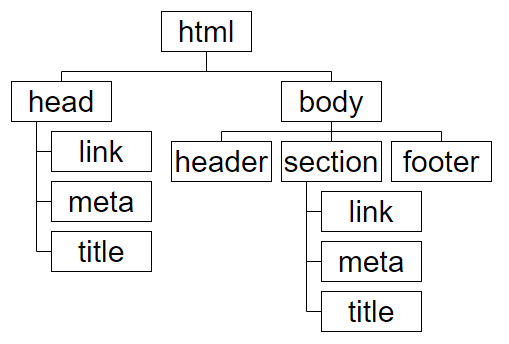
\includegraphics[width=130mm]{img/simple-dom-1.png}
	\caption{Пример DOM-представления для простого HTML документа}
	\label{fig:simple-dom-1}
\end{figure}

Все эти теги не являются уникальными, и в одном документе может быть по несколько экземпляров каждого из них.

В \codeword{body} могут находиться разнообразные элементы.
Например, в родительском \codeword{body} --- дочерний элемент \codeword{header}, в элементе \codeword{header} --- дочерний элемент \codeword{section}, в родительском \codeword{section} --- дочерний \codeword{div}, в \codeword{div} --- элемент \codeword{h3}, и, наконец, в \codeword{h3} — элемент \codeword{span}.
В этом случае \codeword{span} не имеет дочерних элементов, но их можно добавить в любой момент.
Пример того, как можно описать добавление данных элементов, представлен на рисунке \ref{fig:simple-dom-2}.

\begin{figure}[h]
	\centering
	\captionsetup{justification=centering}
	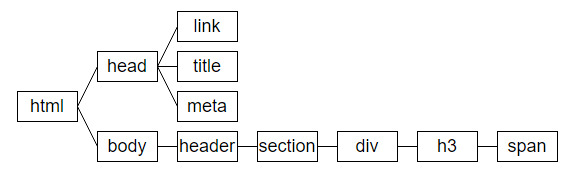
\includegraphics[width=120mm]{img/simple-dom-2.png}
	\caption{Пример DOM-представления для чуть более сложного HTML документа}
	\label{fig:simple-dom-2}
\end{figure}

%Пример, при котором система была бы более разветвлённая и с большим количеством вложений, представлен на рисунке \ref{fig:complicated-dom}.
%
%\begin{figure}[h]
%	\centering
%	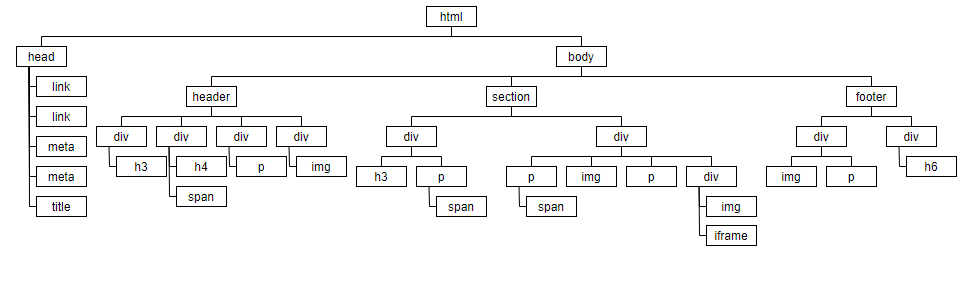
\includegraphics[width=170mm]{img/complicated-dom.png}
%	\caption{Пример DOM-представления для сложного HTML документа}
%	\label{fig:complicated-dom}
%\end{figure}
%
%На схеме изображено довольно большое DOM-дерево, и его сложно воспринимать из-за его размера.
%Для удобства часто используется система многоуровневых списков.
%Пример того, как предыдущее дерево можно преобразовать в такой список, представлен на рисунке \ref{fig:complicated-dom-list}.
%
%\begin{figure}[h]
%	\centering
%	\captionsetup{justification=centering}
%	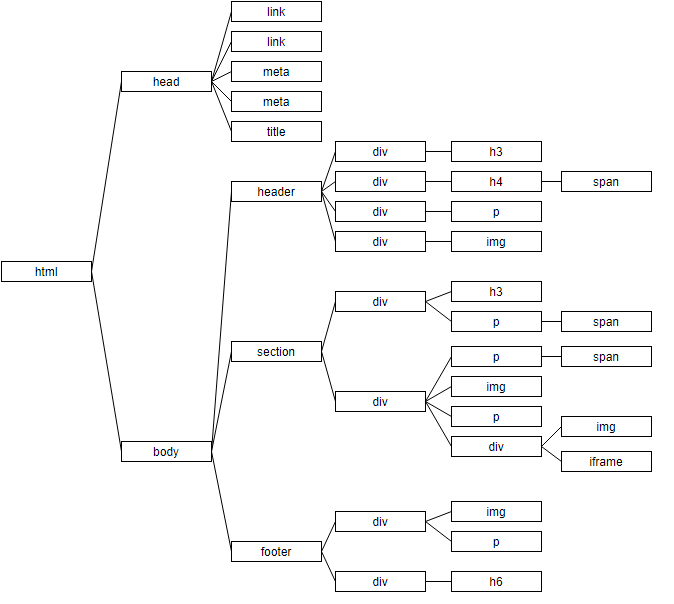
\includegraphics[width=115mm]{img/complicated-dom-list.png}
%	\caption{Пример DOM-представления для сложного HTML документа в виде списка}
%	\label{fig:complicated-dom-list}
%\end{figure}
%
%\clearpage

Элементы могут наследовать не все, но многие свойства своих родителей --- например, цвет, шрифт, видимость, размеры и~т.~д.

Таким образом, чтобы задать стиль шрифта на всей странице, потребуется не прописывать цвет для каждого элемента, а задать его только для \codeword{body}.
А чтобы изменить наследуемое свойство у дочернего элемента, нужно прописать только ему новые свойства.
Наследование удобно для создания единообразной страницы.
DOM-узлы содержат гораздо больше информации, чем просто данные о дочерних узлах \cite{dom-element}.
Они также содержат информацию о родительском узле, стилях, обработчиках событий и свойствах элемента, его исходном  коде и~т.~д.
В таких браузерах, как Google Chrome, DOM-дерево страницы можно посмотреть, например, при помощи инструментов разработчика \cite{devtools}.

%\subsubsection{Алгоритм построения документа с использованием  DOM}
%
%Рассмотрим алгоритм построения DOM-дерева по имеющемуся HTML документу.
%
%Для того, чтобы построить дерево объектной модели, требуется обработать документ и произвести операцию вставки в получающееся дерево $n$ раз, где $n$ - количество элементов.

\subsubsection{Обновления документа с использованием DOM}

Обновление структуры DOM --- распространённая и часто используемая операция, производимая, например, в случае, когда документ должен меняться в ответ на действия пользователя (любая активность на странице).

Рекоммендация W3C в таком случае призывает повторно отрисовать обновлённое дерево с нуля --- то есть, каждый раз, когда необходимо обновить дерево, будет использоваться алгоритм отображения~\cite{reflow}: DOM-дерево строится заново и производится операция вставки элемента $n$ раз, где $n$ - количество элементов.

Благодаря тому, что современные браузеры реализуют DOM и предоставляют API для взаимодействия с DOM-деревом, фреймворки, такие, как Angular, используют именно этот API в своих готовых решениях \cite{angular}. 

\subsection{Алгоритмы, использующие рендеринг на стороне сервера}

Рендеринг на стороне сервера (англ. \textit{Server Side Rendering} --- SSR) --- метод разработки программного обеспечения в web-приложении, которое обрабатывает запросы от пользователя на сервере, который исполняет алгоритмы в соответствии с потребностями бизнеса, отправляя пользователю ответ как результат работы почти со всем процессом рендеринга~\cite{ssr}.

SSR подразумевает, что при обращении к web-странице пользователь получает HTML страницу, работающую согласно одному из HTML стандартов. В данной работе алгоритмы, использующие SSR, не будут рассмотрены подробно, поскольку использование SSR помогает ускорить загрузку страниц, но не обновление их содержимого~\cite{ssr}, алгоритм обновления эквивалентен алгоритму обновления, использующему объектную модель документа, рассмотренную выше. 

Таким образом, при обновлении гипертекстовых документов с использованием SSR используется рекомендованный W3C алгоритм обновления с использованием DOM, поэтому имеет смысл рассматривать именно алгоритм обнвления с использованием DOM.

\subsection{Алгоритмы, использующие виртуальную объектную модель документа}

Основной проблемой DOM является то, что он никогда не был приспособлен для динамического интерфейса~\cite{not-dynamic}.
Он предоставляет удобный программный интерфейс, позволяющий взаимодействовать с ним из кода, но это не решает проблем с производительностью.
Современные социальные сети, такие, как ВКонтакте, Twitter или Facebook будут использовать тысячи DOM узлов, взаимодействие с которыми может занимать ощутимое для пользователя время, в то время как создатели браузера Google Chrome, к примеру, рекомендуют~\cite{dom-max} не использовать в одной странице более 800 узлов.

Одним из решений данной проблемы служит технология виртуальной объектной модели, которая, хоть  и не является стандартом, позволяет по-прежнему взаимодействовать с DOM, но делать это как можно реже.

Виртуальная объектная модель документа (англ. \textit{Virtual Document Object Model} --- VDOM)~\cite{vdom} ---  концепт программирования, в которой идеальное (<<виртуальное>>) представление пользовательского интерфейса хранится в памяти и синхронизуется с <<настоящим>> DOM при помощи алгоритмов согласования.

Вместо того, чтобы работать с DOM напрямую, согласно концепции\break VDOM работа происходит с его легковесной копией, хранящийся непосредственно в памяти компьютера.
За счёт этого операции вставки, сравнения, удаления и обхода узлов дерева происходит быстрее благодаря отсутствию необходимости отрисовывать изменения после каждой операции.

Когда в пользовательский интерфейс добавляются новые элементы, создаётся виртуальная модель DOM, представленная в виде дерева.
Если состояние любого из элементов изменяется, создаётся новое виртуальное дерево DOM.
Затем это дерево сравнивается с предыдущим виртуальным деревом.


Рассмотрим, как для простого  HTML документа, представленного на листинге \ref{code:dom-to-vdom-html}, осуществляется представление DOM- (рисунок \ref{fig:dom-to-vdom-dom}) и VDOM-дерева (листинг \ref{code:dom-to-vdom-vdom}).

\begin{code}
	\captionsetup{justification=raggedright,singlelinecheck=off,margin=4mm}
	\captionof{listing}{Простой HTML документ}
	\label{code:dom-to-vdom-html}
	\inputminted
	[
	frame=single,
	framerule=0.5pt,
	framesep=20pt,
	fontsize=\small,
	tabsize=4,
	linenos,
	numbersep=5pt,
	xleftmargin=10pt,
	]
	{text}
	{code/dom-to-vdom.html}
\end{code}

\begin{figure}[h]
	\centering
	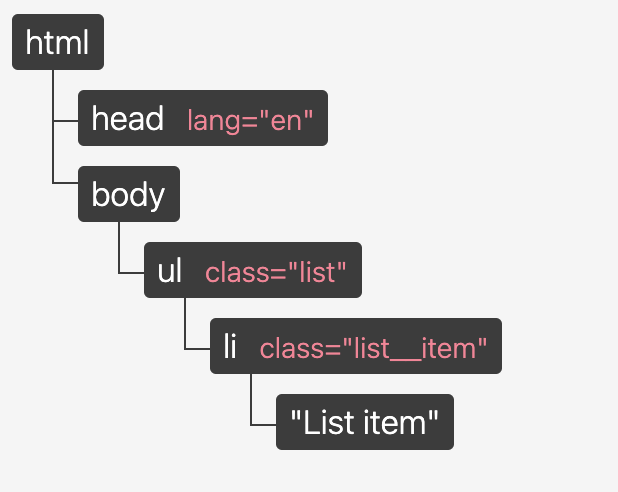
\includegraphics[width=140mm]{img/dom-to-vdom-dom.png}
	\caption{DOM-дерево для простого HTML документа}
	\label{fig:dom-to-vdom-dom}
\end{figure}

\begin{code}
	\captionsetup{justification=raggedright,singlelinecheck=off,margin=4mm}
	\captionof{listing}{VDOM-дерево для простого HTML документа}
	\label{code:dom-to-vdom-vdom}
	\inputminted
	[
	frame=single,
	framerule=0.5pt,
	framesep=20pt,
	fontsize=\small,
	tabsize=4,
	linenos,
	numbersep=5pt,
	xleftmargin=10pt,
	]
	{text}
	{code/dom-to-vdom-vdom.js}
\end{code}

Данный пример служит лишь для демонстрации того, как может осуществляться представление VDOM.
Реальные деревья содержат намного большее число узлов~\cite{dom-element}, а элементы DOM имеют гораздо больше полей (классы, идентификаторы, стили, обработчики событий, поля данных, типы и значения, вспомогательные поля и~т.~п.), и тем не менее содержат гораздо меньше информации, чем узлы DOM за счёт того, что нет необходимости хранить данные, помогающие визуализировать элемент (за это отвечает DOM).

Существует несколько способов использовать VDOM для оптимизации алгоритма отображения гипертекстового документа. с использованием алгоритма согласования и с использованием Fiber алгоритма.

\subsubsection{Обновление документа с использованием VDOM и алгоритма согласования}

Если состояние любого из элементов необходимо изменить, создаётся новое виртуальное дерево.
Затем получившееся дерево сравнивается с предыдущим виртуальным деревом объектной модели документа и происходит вычисления наилучшего из возможных методов внесения изменений в реальной DOM.
Это гарантирует минимальное количество операций с реальной DOM, что приводит к снижении стоимости обновления реальной модели.

На рисунке \ref{fig:vdom-example} показано виртуальное дерево DOM и процесс сравнения.

\begin{figure}[h]
	\centering
	\captionsetup{justification=centering}
	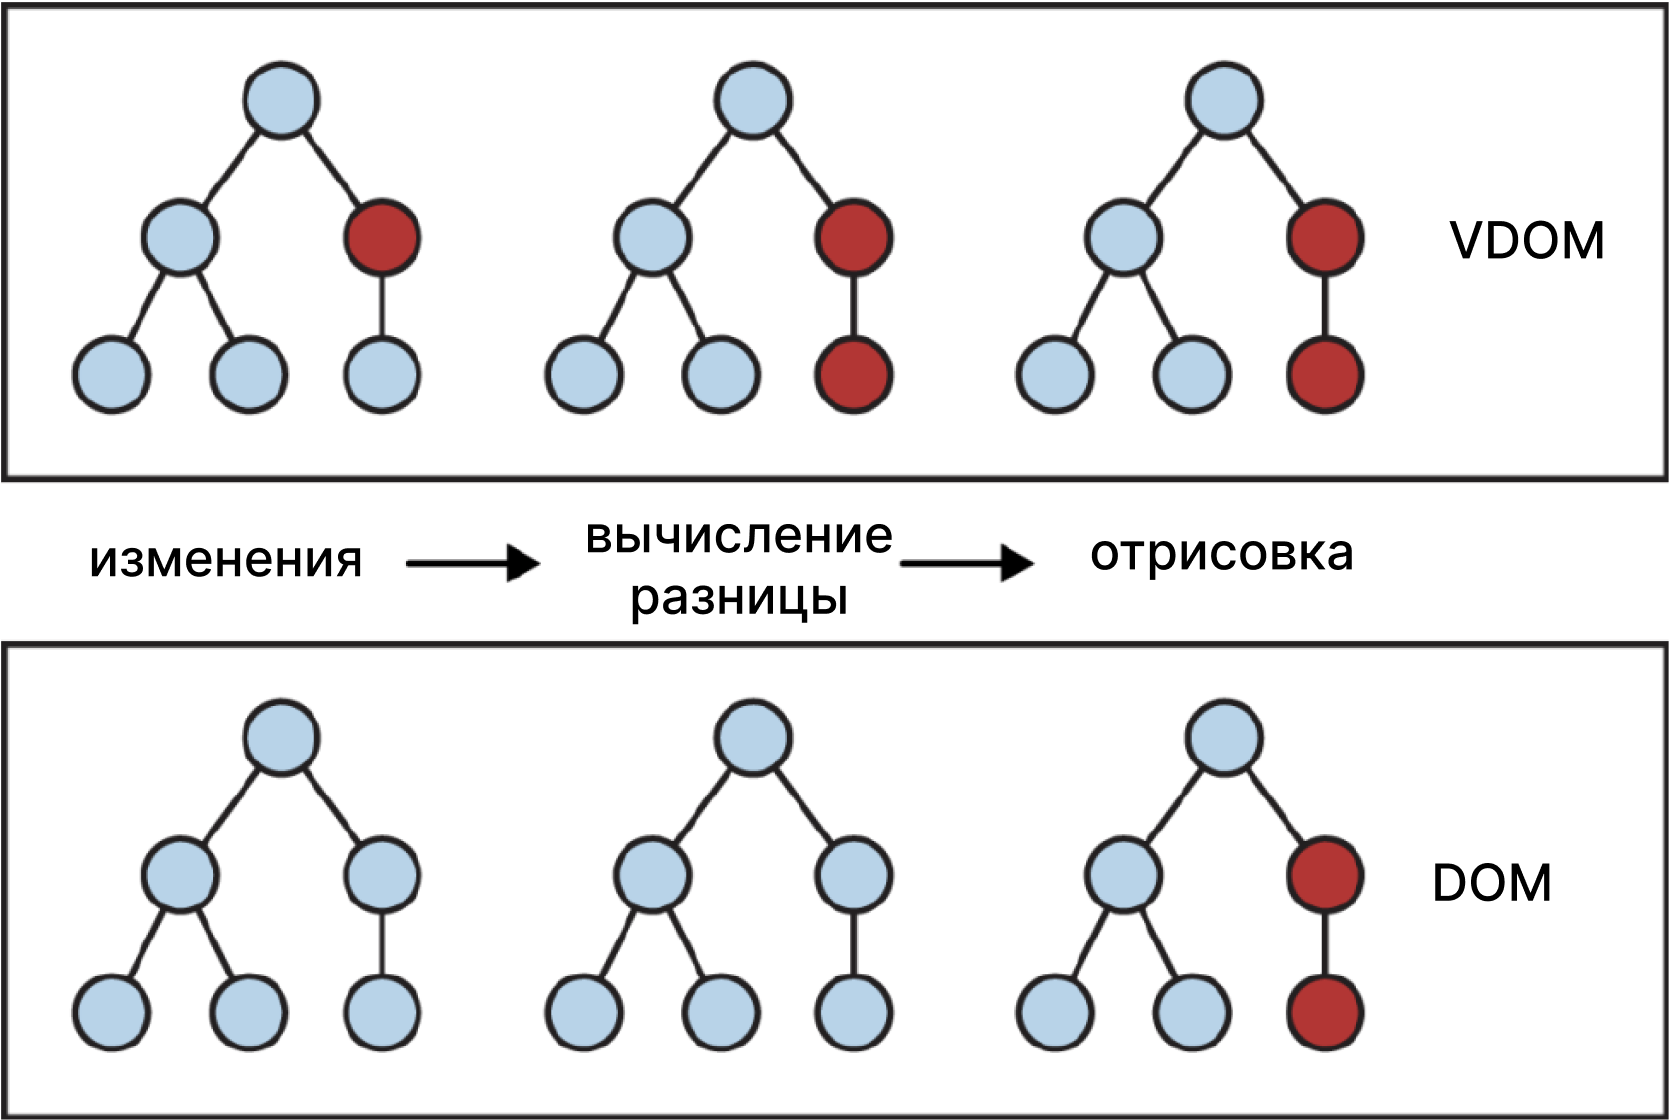
\includegraphics[width=130mm]{img/vdom-example.png}
	\caption{Пример работы алгоритма обновления документа при помощи VDOM}
	\label{fig:vdom-example}
\end{figure}

Красными кружками обозначены узлы, которые изменились --- эти узлы представляют собой элементы пользовательского интерфейса, состояние котоых изменилось.
Затем вычисляется разница между предыдущей версией\break VDOM-дерева и текущей (посредством алгоритма согласования), после чего всё родительское поддерево повторно визуализируется для получения обновлённого пользовательского интерфейса.

\subsubsubsection{Алгоритм согласования}

Алгоритм согласования (англ. \textit{reconciliation})~\cite{reconciliation} --- эвристический алгоритм решения проблемы трансформации одного дерева в другое за минимальное число операций.
Он основан на следующих двух предположениях:

Во-первых, два элемента с разыми типами произведут разные деревья.

Во-вторых, можно указать, какие дочерние элементы могут оставаться стабильными между разными отображениями при помощи специального параметра \codeword{key}.

При сравнении двух деревьев первым делом производится сравнение родительских элементов, начиная с корневого.
Дальнейшее поведение различается в зависимости от типов родительских элементов.

Всякий раз, когда родительские элементы имеют различные типы, старое VDOM-дерево уничтожается и с нуля строится новое.
Так, переходы от \codeword{<div>} к \codeword{<a>} или от \codeword{<img>} к \codeword{<div>} приведут к полному перестроению дерева, старое DOM-дерево также уничтожается.

Любые элементы, лежащие ниже родительского, будут уничтожены, а их состояние уничтожится.
На листиге \ref{code:reconciliation-diff-types} приведён пример изменения узла, при котором меняется его тип и всё поддерево уничтожается.

\begin{code}
	\captionsetup{justification=raggedright,singlelinecheck=off,margin=4mm}
	\captionof{listing}{Пример HTML-узлов разного типа, при сравнении которых деревья будут полностью перестроены}
	\label{code:reconciliation-diff-types}
	\inputminted
	[
	frame=single,
	framerule=0.5pt,
	framesep=20pt,
	fontsize=\small,
	tabsize=4,
	linenos,
	numbersep=5pt,
	xleftmargin=10pt,
	]
	{text}
	{code/reconciliation-diff-types.html}
\end{code}

При сравнении DOM-элементов одного типа, алгоритм согласования проверяет их атрибуты, сохраняет лежащий в основе элементов DOM-узел и обновляет только изменённые атрибуты (пример таких элементов приведён на листинге \ref{code:reconciliation-same-types}).

\begin{code}
	\captionsetup{justification=raggedright,singlelinecheck=off,margin=4mm}
	\captionof{listing}{Пример HTML-узлов одного типа, при сравнении которых будет сохранена лишь разница содержимого атрибутов}
	\label{code:reconciliation-same-types}
	\inputminted
	[
	frame=single,
	framerule=0.5pt,
	framesep=20pt,
	fontsize=\small,
	tabsize=4,
	linenos,
	numbersep=5pt,
	xleftmargin=10pt,
	]
	{text}
	{code/reconciliation-same-types.html}
\end{code}

При рекурсивном обходе дочерних элементов DOM-узла алгоритм согласования проходит по спискам потомков одновременно и находит отличие.
Например, при добавлении элемента в конец дочерних элементов, преобразование между этими деревьями работает хорошо, определяя минимальный набор операций.

\begin{code}
	\captionsetup{justification=raggedright,singlelinecheck=off,margin=4mm}
	\captionof{listing}{Пример HTML-узлов при добавлении элемента в конец дочернего}
	\label{code:reconciliation-add-to-end}
	\inputminted
	[
	frame=single,
	framerule=0.5pt,
	framesep=20pt,
	fontsize=\small,
	tabsize=4,
	linenos,
	numbersep=5pt,
	xleftmargin=10pt,
	]
	{text}
	{code/reconciliation-add-to-end.html}
\end{code}

Алгоритм согласования сравнит два дерева \codeword{<li>первый</li>}, сравнит два дерева \codeword{<li>второй</li>}, а затем вставит дерево \codeword{<li>третий</li>}.

При вставке элемента в начало, прямолинейная реализация такого алгоритма будет работать не эффективно. Например, преобразование между этими деревьями работает плохо, минимальный набор операций для преобразованя одного дерева в другое не будет найден.

Алгоритм согласования будет преобразовывать каждого потомка, вместо того, чтобы оставить элементы \codeword{<li>Санкт-Петербург</li>} и \linebreak
\codeword{<li>Москва</li> }. Пример таких узлов продемонстрирован на листинге  \ref{code:reconciliation-add-to-start}.

\begin{code}
	\captionsetup{justification=raggedright,singlelinecheck=off,margin=4mm}
	\captionof{listing}{Пример HTML-узлов при добавлении элемента в начало дочернего}
	\label{code:reconciliation-add-to-start}
	\inputminted
	[
	frame=single,
	framerule=0.5pt,
	framesep=20pt,
	fontsize=\small,
	tabsize=4,
	linenos,
	numbersep=5pt,
	xleftmargin=10pt,
	]
	{text}
	{code/reconciliation-add-to-start.html}
\end{code}

Для решения этой проблемы существуют вспомогательные атрибуты \codeword{key} --- ключи~\cite{keys}. Когда у дочерних элементов есть ключи, алгоритм согласования использует их, чтобы сопоставить потомков исходного виртуального дерева с потомками полученного виртуального дерева.

Значение атрибута \codeword{key} при этом должно быть уникальным.
Так, как значение ключа  можно использовать уникальный идентификатор элемента, если он есть, или же можно добавить новое свойство идентификатора или прохешировать данные, чтобы сгенерировать ключ.
Достаточно, чтобы ключ элемента был уникальным среди его соседей, а не глобально.

Например, если добавить \codeword{key} к примеру выше, преобразование дерева будет верным.
\newline

\begin{code}
	\captionsetup{justification=raggedright,singlelinecheck=off,margin=4mm}
	\captionof{listing}{Пример HTML-узлов при добавлении элемента в начало дочернего с использованием ключей}
	\label{code:reconciliation-add-to-start-keys}
	\inputminted
	[
	frame=single,
	framerule=0.5pt,
	framesep=20pt,
	fontsize=\small,
	tabsize=4,
	linenos,
	numbersep=5pt,
	xleftmargin=10pt,
	]
	{text}
	{code/reconciliation-add-to-start-keys.html}
\end{code}

Алгоритм согласования является эвристическим~\cite{euristic} алгоритмом, и если предположения, на которых он основан, не соблюдены, пострадает производительность.

Так, алгоритм не будет пытаться сопоставить поддеревья элементов разных типов, а ключи должны быть стабильными (например, ключ, произведённый случайно, не является стабильным), предсказуемым и уникальным.
Нестабильные ключи вызовут необязательное пересоздание многих экземпляров элемента и DOM-узлов, что может вызывать ухудшение производительности и потерю состояния у дочерних элементов.


\subsubsection{Обновление документа с использованием Fiber алгоритма}

Fiber --- основной алгоритм сравнения библиотеки React, начиная с 16 версии конкурирующий с алгоритмом согласования~\cite{fiber}. Для пользовательского интерфейса не важно, чтобы каждое обновление было применено сразу; фактически такое поведение будет лишним, оно будет способствовать падению количества кадров в секунду и ухудшению пользовательского опыта~\cite{react-dive}. 

Волокно (англ. \textit{fiber}) --- объект, являющийся абстракцией работы, которую необходимо выполнить~\cite{react-dive}. Работой являются любые вычисления, которые должны быть выполнены для того, чтобы определить, какие объекты необходимо обновлять, а какие можно оставить в прежнем состоянии. Такая работа должна иметь возможность быть остановленной и возобновлённой. Рассмотрим следующий пример: пусть имеются HTML-элементы, представленные на листинге \ref{code:fiber-1}.

\begin{code}
	\captionsetup{justification=raggedright,singlelinecheck=off,margin=4mm}
	\captionof{listing}{Пример HTML-элементов для демонстрации структуры волокна}
	\label{code:fiber-1}
	\inputminted
	[
	frame=single,
	framerule=0.5pt,
	framesep=20pt,
	fontsize=\small,
	tabsize=4,
	linenos,
	numbersep=5pt,
	xleftmargin=10pt,
	]
	{text}
	{code/fiber-1.html}
\end{code}

Волокно, отвечающее за вычисления, связанные с кнопкой, имеющий класс btn, будет иметь следующий вид, представленный на листинге \ref{code:fiber-1-js}.

\begin{code}
	\captionsetup{justification=raggedright,singlelinecheck=off,margin=4mm}
	\captionof{listing}{Fiber объект для элемента кнопки}
	\label{code:fiber-1-js}
	\inputminted
	[
	frame=single,
	framerule=0.5pt,
	framesep=20pt,
	fontsize=\small,
	tabsize=4,
	linenos,
	numbersep=5pt,
	xleftmargin=10pt,
	]
	{text}
	{code/fiber-1.js}
\end{code}

Поля объекта, представленного на листинге \ref{code:fiber-1-js}, имеют следующий смысл:
\begin{enumerate}[label=\arabic*)]
	\item stateNode --- указатель на объект DOM-дерева, соответствующего элементу волокна (в данном случае кнопке);
	\item child --- указатель на волокно первого дочернего элемента (в данном случае дочерних элементов нет);
	\item return --- указатель на волокно родительского элемента (в данном слечае список);
	\item sibling --- указатель на первый соседний элемент (в данном случае элемент div).
\end{enumerate}


\subsection*{Вывод}

В данном разделе были рассмотрены принципы работы с гипертекстовыми документами согласно объектной модели документа (DOM) и витруальной объектной модели документа (VDOM) и проведено их сравнение.
Также был рассмотрен алгоритм согласования, находящий минимальный набор операций, необходимых для преобразования одного дерева в другое.
В соответствии с поставленной целью, необходимо разработать алгоритмы обновления документа с использованием DOM и VDOM, а также алгоритма согласования.

На вход алгоритма обновления с использованием DOM будут подаваться обрабатываемый элемент, изменяемый элемент и элемент, который нужно отрисовать вместо него.
На вход алгоритма обновления документа с использованием VDOM будут подаваться корни старого VDOM-дерева и нового VDOM-дерева, а на вход алгоритма согласования - обрабатываемые узлы старого и нового VDOM-деревьев, а также указатели на массивы изменений узлов и поддеревьев,